\documentclass[11pt,a4paper]{article}

% ---------------------------------------------------------------------------
% Benchmarking Homomorphic Encryption — Project Summary Report (Group 7)
% Single-column article. Compile with:  tectonic FINAL_REPORT.tex
% ---------------------------------------------------------------------------

\usepackage[T1]{fontenc}
\usepackage[utf8]{inputenc}
\usepackage{lmodern}
\usepackage[margin=1in]{geometry}
\usepackage{graphicx}
\usepackage{booktabs}
\usepackage{tabularx}
\usepackage{array}
\usepackage{amsmath}
\usepackage{amssymb}
\usepackage{siunitx}
\usepackage{xcolor}
\usepackage{listings}
\usepackage{caption}
\usepackage{enumitem}
\usepackage{float}
\usepackage[hidelinks]{hyperref}

\graphicspath{{../figures/}{figures/}}

% --- colours -----------------------------------------------------------------
\definecolor{accent}{HTML}{9A6B3F}      % warm sand accent
\definecolor{rule}{HTML}{C9B79C}
\definecolor{codebg}{HTML}{F5F0E8}
\definecolor{codeframe}{HTML}{D8CBB4}

% --- listings ----------------------------------------------------------------
\lstset{
  basicstyle=\ttfamily\small,
  backgroundcolor=\color{codebg},
  frame=single,
  rulecolor=\color{codeframe},
  framesep=6pt,
  xleftmargin=6pt,
  breaklines=true,
  columns=fullflexible,
  keepspaces=true,
  showstringspaces=false,
}

% --- callout box (framed) ----------------------------------------------------
\newcommand{\keyfinding}[1]{%
  \begin{center}
  \fcolorbox{rule}{codebg}{%
    \parbox{0.94\linewidth}{\vspace{2pt}\textbf{Key finding.} #1\vspace{2pt}}}
  \end{center}}

\captionsetup{font=small,labelfont=bf}
\setlength{\parskip}{0.35em}
\setlength{\parindent}{0pt}

% --- title metadata ----------------------------------------------------------
\title{\vspace{-1.2cm}\textbf{Benchmarking Homomorphic Encryption}\\[0.3em]
  \large A Reproducible Study of the Overhead of Computing on Encrypted Data}
\author{%
  Bar Pesso \quad\textbullet\quad Shay Harush \quad\textbullet\quad Shon Platok\\[0.4em]
  \textbf{Group 7} \quad\textbullet\quad Course: Confidential Computing}
\date{July 2026}

\begin{document}
\maketitle
\thispagestyle{empty}

% ============================================================================
\begin{abstract}
\noindent
Homomorphic Encryption (HE) allows computation directly on encrypted data, a
capability that conventional ciphers such as AES and RSA do not provide. This
project builds a \emph{reproducible} benchmark that measures the practical
overhead of HE for simple numerical analytics --- runtime, ciphertext size, and
correctness --- against AES-256 and RSA-2048 baselines, and frames the
comparison honestly. The central result, measured on a dataset of
\num{100000} records, is one line: computing a sum the traditional way costs
$\sim$\SI{0.16}{\milli\second} but exposes the plaintext to the compute party,
whereas computing the same sum homomorphically costs $\sim$\SI{500}{\milli\second}
and never exposes the data. HE is therefore roughly three orders of magnitude
slower for this task, carries a $\sim$$10\times$ ciphertext-size overhead, and
requires a fixed $\sim$\SI{34}{\mega\byte} of keys before any computation begins
--- yet it is the only one of the three schemes that keeps data encrypted
\emph{during} processing. This report quantifies exactly when that trade is
worth making, documents the design decisions behind the benchmark, and delivers
a fully reproducible artifact (Docker image, test suite, and interactive
dashboard).
\end{abstract}

\tableofcontents
\newpage

% ============================================================================
\section{Introduction and Motivation}

Confidential computing addresses a gap left by conventional cryptography. AES and
RSA protect data \textbf{at rest} and \textbf{in transit}, but to \emph{compute}
on that data it must first be decrypted, exposing it to whoever runs the
computation. Homomorphic Encryption removes that exposure by computing on
ciphertext directly: an untrusted server can evaluate a function over encrypted
inputs and return an encrypted result that only the key holder can open.

This property --- protecting data \textbf{in use} --- is attractive for
outsourced analytics, cross-organisation aggregation, and privacy-preserving
machine learning. But HE has a reputation for being impractically expensive, and
that reputation is usually asserted rather than measured. The motivation for this
project is to replace hand-waving with numbers: to build a small, honest,
reproducible benchmark that shows \emph{exactly} what HE costs for the simplest
useful workload (numerical aggregation) and lets a reader judge for themselves
when the cost is justified.

We deliberately keep the scope narrow --- four numerical operations, one HE
scheme, synthetic data --- because a narrow scope executed rigorously and
reproducibly is more useful than a broad survey of unverified numbers. Every HE
result in this report is checked against a plaintext reference, every timing is
the mean of five repeats after a warm-up, and the full environment is captured
alongside the results so the numbers can be regenerated.

% ============================================================================
\section{Objectives and Research Question}

\paragraph{Research question.}
\emph{For basic numerical operations, what overhead does HE add in runtime,
memory, ciphertext size, and correctness --- and when is that overhead
acceptable?}

\paragraph{Concrete objectives.} The project set out to:
\begin{enumerate}[leftmargin=1.4em,itemsep=1pt]
  \item Implement an HE pipeline (encrypt $\rightarrow$ compute on ciphertext
    $\rightarrow$ decrypt) for addition, multiplication, sum, and average using
    the CKKS scheme.
  \item Implement AES-256 and RSA-2048 baselines for a fair, honestly-framed
    comparison.
  \item Measure runtime, ciphertext size, approximation error, and scalability
    up to \num{100000} records, verifying every HE result against a plaintext
    ground truth.
  \item Package everything reproducibly (seeded data, pinned dependencies,
    Docker, a test suite) and communicate the findings through a written report
    and an interactive dashboard.
\end{enumerate}

% ============================================================================
\section{The Fundamental Asymmetry (Why This Comparison Is ``Unfair'' by Design)}
\label{sec:asymmetry}

The most important framing of this project is that \textbf{comparing HE to
AES/RSA is inherently unfair, because they solve different problems.} Stating
runtime numbers without this frame would be misleading.

\begin{table}[H]
\centering
\caption{The three schemes protect different states of data.}
\begin{tabularx}{\linewidth}{Xcc}
\toprule
\textbf{Property} & \textbf{AES-256 / RSA-2048} & \textbf{CKKS (HE)}\\
\midrule
Protects data \textbf{at rest}                 & Yes & Yes\\
Protects data \textbf{in transit}              & Yes & Yes\\
Protects data \textbf{in use} (during compute) & \textbf{No} & \textbf{Yes}\\
Can compute on ciphertext                      & \textbf{No} & \textbf{Yes}\\
\bottomrule
\end{tabularx}
\end{table}

To analyse AES- or RSA-protected data you must \textbf{decrypt it first}, perform
the computation on plaintext, then optionally re-encrypt. During that computation
the data is fully exposed to the compute party. HE computes on the ciphertext and
only the final result is decrypted, by the key holder.

Consequently this report does \textbf{not} claim HE is ``better'' than AES or
RSA. It measures the \textbf{cost of a capability that AES and RSA simply do not
have.} Every result below should be read as the price of keeping data encrypted
while it is being used.

% ============================================================================
\section{Project Planning and Approach}

The work was organised around a single principle stated in the project charter:
\emph{reproducibility is the deliverable, not an afterthought}. That principle
drove the sequencing of the work into five phases.

\begin{table}[H]
\centering
\caption{Project phases and their outputs.}
\begin{tabularx}{\linewidth}{@{}p{0.5cm}p{3.3cm}X@{}}
\toprule
\# & \textbf{Phase} & \textbf{Output}\\
\midrule
1 & Foundation & Pinned Python 3.11 environment, Docker image, seeded
    synthetic-data generator, plaintext NumPy reference, timing/metrics harness.\\
2 & HE core & CKKS context and key generation, chunked packed encryption,
    add/multiply/sum/mean on ciphertext, decryption, size accounting.\\
3 & Baselines & AES-256-GCM and RSA-2048-OAEP protection paths, with the
    fair-comparison rules (\S\ref{sec:methodology}) enforced in code.\\
4 & Measurement & Benchmark orchestrator over
    size~$\times$~operation~$\times$~scheme; depth-sweep experiment; figure and
    CSV generation; \texttt{run\_config.json} capture.\\
5 & Communication & Test suite, interactive Streamlit dashboard, and this
    written report.\\
\bottomrule
\end{tabularx}
\end{table}

\paragraph{Controlled-comparison design.} A deliberate planning decision was that
the \textbf{same synthetic data is encrypted under all three schemes}. This is a
controlled comparison --- methodologically stronger than benchmarking each scheme
on unrelated data --- and it means differences in the results are attributable to
the schemes, not to the inputs.

\paragraph{Risk management.} Two risks were identified early and handled in the
plan rather than discovered late: (i)~TenSEAL ships no wheel for Python~3.13 and
requires NumPy~$<2.0$ for ABI compatibility, so the environment was pinned to
Python~3.11 from the start; and (ii)~process-level memory measurement was
expected to be unreliable for a C++-backed library, so ciphertext size was
designated the authoritative size signal up front (borne out in
\S\ref{sec:limitations}).

% ============================================================================
\section{Solution Choices and Rationale}
\label{sec:choices}

Every tool and parameter was chosen for a stated reason; the choices are the
substance of the ``considerations behind the solution'' the reviewer asked for.

\subsection{Technology stack}

\begin{table}[H]
\centering
\caption{Technology choices and rationale.}
\begin{tabularx}{\linewidth}{@{}p{2.6cm}p{2.7cm}X@{}}
\toprule
\textbf{Layer} & \textbf{Choice (version)} & \textbf{Rationale}\\
\midrule
Language        & Python 3.11        & TenSEAL ships no 3.13 wheel; 3.11 pinned for the wheel and NumPy ABI.\\
HE library      & TenSEAL 0.3.16 (CKKS) & Easiest HE library for a Python prototype; NumPy-friendly tensor API.\\
Classical crypto& cryptography 42.0.8 & Standard, audited AES-256-GCM and RSA-2048-OAEP primitives.\\
Numerics        & NumPy 1.26.4       & Plaintext reference + seeded data; pinned $<2.0$ for TenSEAL ABI.\\
Data handling   & pandas 2.2.2       & CSV analysis and dashboard tables.\\
Plotting        & matplotlib 3.8.4   & Headless (Agg) figure generation.\\
System metrics  & psutil 5.9.8       & Process RSS (TenSEAL ciphertexts live in C++ memory, invisible to \texttt{tracemalloc}).\\
Tests           & pytest 8.2.2       & Correctness, metrics, security, app smoke tests.\\
UI              & Streamlit 1.37.1 + Plotly & Interactive dashboard / live demo / use case.\\
Runtime         & Docker $+$ compose & \texttt{python:3.11-slim} base; full reproducibility; results/figures bind-mounted to host.\\
\bottomrule
\end{tabularx}
\end{table}

\subsection{Why CKKS?}

CKKS was chosen because it operates on \textbf{real-valued vectors} and supports
division by a constant, which covers all four target operations including the
average (mean $=$ sum $\times\,1/N$). CKKS is an \textbf{approximate} scheme, so
every decrypted result is compared against an exact plaintext reference and its
error is reported. The alternative exact-integer schemes (BFV/BGV) are noted as
the natural follow-up (\S\ref{sec:limitations}) but were out of scope for a first
benchmark focused on real-valued analytics.

\subsection{CKKS parameters}
\label{sec:params}

We use \texttt{poly\_modulus\_degree = 8192} (4096 usable slots per ciphertext),
\texttt{coeff\_mod\_bit\_sizes = [60, 40, 40, 60]}, and
\texttt{global\_scale} $=2^{40}$. The coefficient-modulus chain totals 200 bits,
within the limit for $\sim$\textbf{128-bit security} at this ring dimension, and
provides two rescaling levels (one to two multiplications; see the measured depth
limit in \S\ref{sec:depth}). Datasets larger than 4096 values are split into
$\lceil N/4096\rceil$ ciphertexts (``chunking''); \texttt{sum} is computed
per-chunk via Galois-key rotations and then combined.

% ============================================================================
\section{Methodology}
\label{sec:methodology}

\subsection{Datasets}

Synthetic numerical data: 1-D arrays of \texttt{float64} values drawn uniformly
from $[0, 100)$, generated with a fixed NumPy seed so every run is reproducible.
Two arrays per size are used --- \texttt{a} (seed 42) and \texttt{b} (seed 43,
the second operand for add/multiply). The \textbf{same data is encrypted under
all schemes}. Sizes benchmarked: \textbf{200, 1{,}000, 10{,}000, and
100{,}000 records}. The data is synthetic and non-sensitive, chosen for
reproducibility and because CKKS is real-valued.

\subsection{Fair-comparison rules and measurement}

Costs are separated into three buckets so no scheme is judged unfairly:
\begin{enumerate}[leftmargin=1.4em,itemsep=1pt]
  \item \textbf{Data protection} --- encryption / decryption (all schemes).
  \item \textbf{Computation} --- HE on ciphertext vs.\ plaintext computation
    (measured separately).
  \item \textbf{Size overhead} --- ciphertext vs.\ plaintext bytes.
\end{enumerate}

Each measurement runs \textbf{five times after a discarded warm-up}; we report
the mean, with standard deviations recorded in the CSV and shown as error bars in
the figures. Timing uses \texttt{perf\_counter}; sub-millisecond calls (AES, RSA,
plaintext NumPy) sit near the timer's practical noise floor, so the harness times
a \emph{batch} of calls per sample and reports the per-call mean --- small
non-monotonicities across sizes in such microsecond figures should be read as
jitter. Correctness is checked against the NumPy reference (exact equality for
AES/RSA round-trips; tolerance for approximate CKKS). The full configuration,
library versions, and machine details are written to \texttt{run\_config.json}.

Two rules prevent misleading baseline numbers: \textbf{RSA-2048-OAEP} can encrypt
at most $\sim$190 bytes, so it cannot encrypt bulk data --- it is measured
\textbf{per single record} and reported as such, never as a bulk figure; and
\texttt{count} is plaintext metadata, not an HE computation, and is labelled
accordingly.

\subsection{Measurement environment}

Runs were executed inside the Docker image on an x86\_64 host (16 logical CPUs,
Linux/WSL2), Python 3.11.15, TenSEAL 0.3.16, NumPy 1.26.4. The environment and
CKKS parameters are recorded in \texttt{results/run\_config.json} so the figures
in this report correspond to a single, captured run.

% ============================================================================
\section{System Architecture and Implementation}

The codebase is deliberately small and modular, with all tunable parameters in a
single \texttt{config.py} so a run is defined by one file plus a seed.

\begin{lstlisting}[caption={Repository layout (core modules).},captionpos=b]
config.py                    # all parameters (sizes, repeats, CKKS params, seed)
he_benchmark/
  data.py                    # seeded synthetic data (uniform float64 in [0,100))
  metrics.py                 # perf_counter timing, peak-RSS sampler, repeat-runner
  reference.py               # plaintext NumPy ground truth
  he_ckks.py                 # CKKS context/keys, chunked encrypt, add/mul/sum/mean
  baseline_aes.py            # AES-256-GCM (data protection only)
  baseline_rsa.py            # RSA-2048-OAEP per-block (data protection only)
  security.py                # qualitative security profiles + takeaways
  environment.py             # library versions / CPU capture
experiments/run_benchmark.py # size x op x scheme -> results.csv + run_config.json
experiments/depth_sweep.py   # CKKS error vs multiplicative depth -> depth_sweep.json
analysis/make_plots.py       # 8 figures + workflow_comparison.csv
app/streamlit_app.py         # 4-tab interactive dashboard
tests/                       # 21 tests (correctness, metrics, security, app smoke)
Dockerfile . docker-compose.yml . requirements.lock . README.md
results/ . figures/          # generated outputs (bind-mounted to host)
\end{lstlisting}

The interactive dashboard reuses the exact same \texttt{he\_benchmark} modules as
the benchmark, so live demo results match the measured pipeline rather than
re-implementing it.

% ============================================================================
\section{Results}

\subsection{Correctness and approximation error}

Every operation decrypted correctly under all schemes. AES and RSA round-trips
are exact. CKKS is approximate; its error is small and \textbf{stable across
dataset sizes}, but differs by operation. We report \textbf{both} the mean
relative error and the maximum absolute error, because the two tell different
stories.

\begin{table}[H]
\centering
\caption{CKKS approximation error by operation (at $N=100{,}000$ for the absolute column).}
\begin{tabularx}{\linewidth}{@{}lccX@{}}
\toprule
\textbf{Operation} & \textbf{Mean rel.\ error} & \textbf{Max abs.\ error} & \textbf{Note}\\
\midrule
Addition       & $\sim$$1.7\times10^{-11}$ & $\sim$$1.4\times10^{-8}$ & Pure addition; relatively very precise.\\
Sum            & $\sim$$2\times10^{-11}$--$6\times10^{-10}$ & $\sim$$1.1\times10^{-4}$ & Additions only; tiny \emph{relative} error, but absolute error grows with the large aggregate.\\
Multiplication & $\sim$$1.3\times10^{-7}$ & $\sim$$1.3\times10^{-3}$ & ct $\times$ ct $+$ rescale sets a $\sim$$10^{-7}$ relative floor.\\
Average (mean) & $\sim$$1.1$--$1.4\times10^{-7}$ & $\sim$$5.4\times10^{-6}$ & $=$ sum $\times(1/N)$; the scalar multiply sets the same $\sim$$10^{-7}$ floor.\\
\bottomrule
\end{tabularx}
\end{table}

\textbf{Reading the table --- a normalisation caveat.} Relative error is
normalised by the result's magnitude, and that magnitude differs by $\sim$5
orders of magnitude across these operations (sum $\approx 5\times10^{6}$ vs.\
mean $\approx 50$). So the apparent gap --- sum at $\sim$$10^{-11}$ versus mean at
$\sim$$10^{-7}$ --- is \textbf{largely a normalisation artifact, not a real
precision difference}: mean is simply sum $\times(1/N)$, so it cannot be ``more
wrong'' than the sum it is built from. \textbf{Absolute error is the more honest
signal for aggregates.} The genuine pattern is by operation \emph{type}: pure
additions (add, sum) are relatively very precise ($\sim$$10^{-11}$), while
operations that include a ciphertext rescale (multiply, mean) share a
$\sim$$10^{-7}$ relative floor. Either way the errors are negligible for
analytics but non-zero, as CKKS requires.

\begin{figure}[H]
\centering
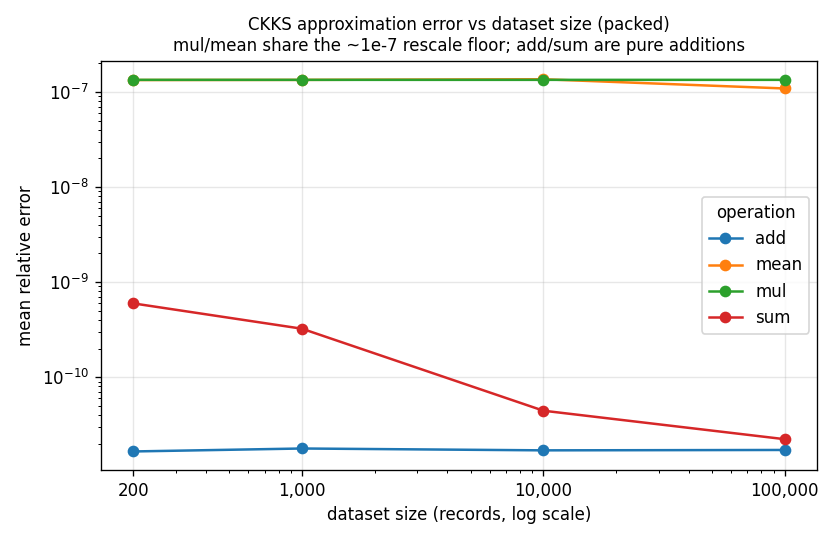
\includegraphics[width=0.78\linewidth]{ckks_error_vs_size.png}
\caption{CKKS approximation error vs.\ dataset size, per operation. The error is
stable across sizes; the separation is by operation type, not by $N$.}
\end{figure}

\subsection{Runtime and scalability}

\begin{table}[H]
\centering
\caption{CKKS runtime (packed, mean over 5 runs), in milliseconds.}
\begin{tabular}{@{}lccccc@{}}
\toprule
$N$ & \textbf{Encrypt} & \textbf{Add} & \textbf{Multiply} & \textbf{Sum} & \textbf{Mean}\\
\midrule
200      & 3.1 & 0.06 & 2.3 & 30  & 33\\
1{,}000  & 2.8 & 0.06 & 2.3 & 65  & 75\\
10{,}000 & 8.7 & 0.14 & 6.6 & 89  & 90\\
100{,}000& 73  & 1.5  & 54  & \textbf{503} & 501\\
\bottomrule
\end{tabular}
\end{table}

Two patterns stand out. First, \textbf{encryption and aggregation dominate}:
\texttt{sum} and \texttt{mean} are far more expensive than element-wise
\texttt{add}/\texttt{multiply} because reducing across slots requires
$\sim$$\log_2(N)$ Galois-key rotations per ciphertext chunk, each costly. Second,
the cost scales with the number of ciphertext chunks --- at $N=100{,}000$ the
data occupies 25 ciphertexts, so per-chunk work multiplies; the headline
\texttt{sum} figure is $503\pm20$~ms (mean~$\pm$~std over the five runs).
Decryption is cheap for a scalar result ($\sim$0.7~ms) but larger for a full
vector result ($\sim$14--20~ms at $N=100{,}000$).

Note that \texttt{mean} is not independent of \texttt{sum}: it is computed as
\texttt{sum} followed by a plaintext scalar multiply, so its cost necessarily
\emph{includes} sum's. The two are therefore near-identical (501 vs.\ 503~ms at
$N=100{,}000$), as expected --- not two separate data points.

\begin{figure}[H]
\centering
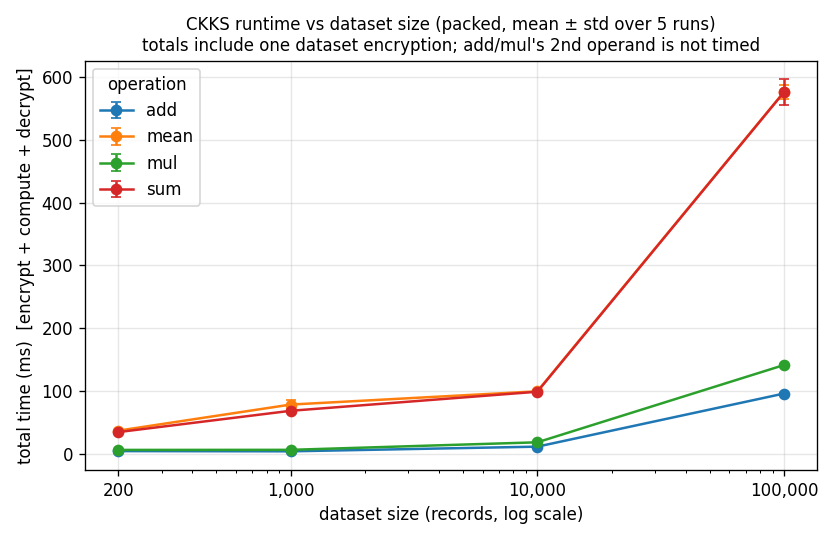
\includegraphics[width=0.72\linewidth]{ckks_runtime_vs_size.png}
\caption{CKKS total time vs.\ dataset size, per operation (log scale).}
\end{figure}

\begin{figure}[H]
\centering
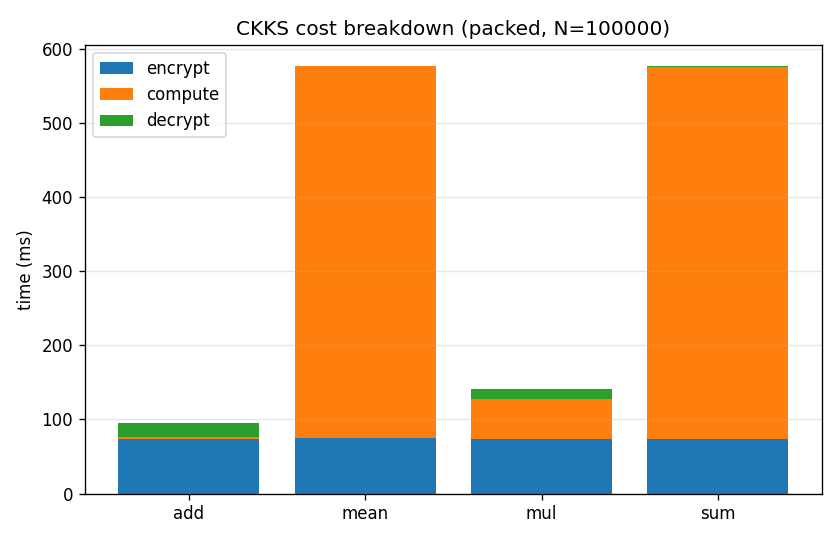
\includegraphics[width=0.72\linewidth]{ckks_cost_breakdown.png}
\caption{Encrypt / compute / decrypt split at the largest size ($N=100{,}000$).
Encryption and aggregation, not decryption, dominate the cost.}
\end{figure}

\subsection{Size overhead --- ciphertext and the fixed key/context cost}

\textbf{Ciphertext size is the authoritative memory/size signal in this report.}
(Process-level peak-memory sampling proved too noisy to report responsibly; see
\S\ref{sec:limitations}.)

\begin{table}[H]
\centering
\caption{Encrypted dataset vs.\ raw plaintext.}
\begin{tabular}{@{}lccccc@{}}
\toprule
$N$ & \textbf{Plaintext} & \textbf{CKKS ciphertext} & \textbf{Chunks} & \textbf{Overhead}\\
\midrule
200       & 1.6 KB & 334 KB  & 1  & $\sim$$209\times$\\
1{,}000   & 8 KB   & 334 KB  & 1  & $\sim$$42\times$\\
10{,}000  & 80 KB  & 1.0 MB  & 3  & $\sim$$12.5\times$\\
100{,}000 & 800 KB & 8.36 MB & 25 & $\sim$$10.4\times$\\
\bottomrule
\end{tabular}
\end{table}

A subtle but important finding: \textbf{a single CKKS ciphertext is
$\sim$334~KB regardless of how many of its 4{,}096 slots are filled.} Small
datasets therefore waste most of a ciphertext, which is why the overhead ratio is
enormous at $N=200$ ($\sim$$209\times$) and falls toward $\sim$$10\times$ only
once the data is large enough to fill the slots. By contrast, AES adds just
\textbf{28 bytes} (a 12-byte nonce plus a 16-byte authentication tag) to the
plaintext, at any size.

\keyfinding{Before any value is encrypted or any computation is run, the public
context --- public key plus Galois keys (rotations) and relinearization keys
(multiplication) --- is $\approx$\SI{34}{\mega\byte}
(\num{35476814}~bytes; 33.8~MiB), \emph{independent of dataset size}. For a
dataset of 200 records the keys outweigh the encrypted data by $\sim$$100\times$.
This fixed cost, frequently overlooked, is what makes HE impractical for small or
latency-sensitive workloads.}

\begin{figure}[H]
\centering
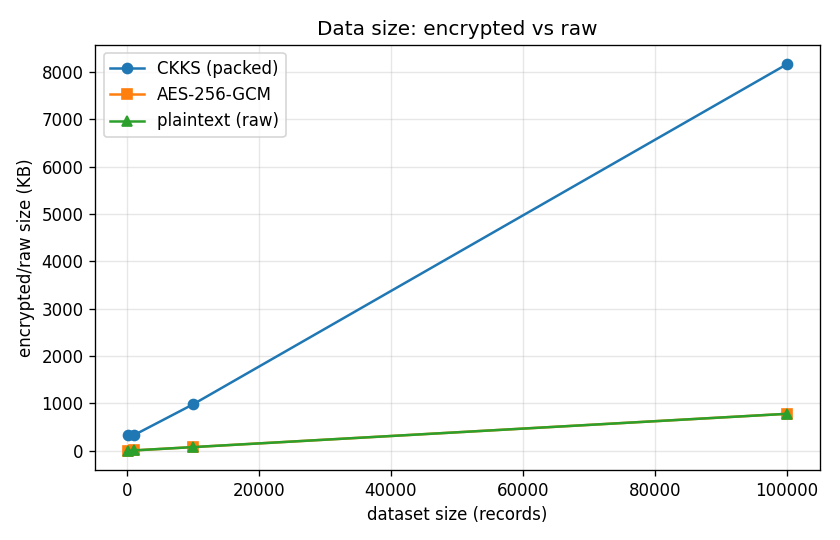
\includegraphics[width=0.72\linewidth]{ciphertext_size_vs_size.png}
\caption{Encrypted vs.\ raw data size across dataset sizes.}
\end{figure}

\subsection{Packing: why batching is mandatory}

CKKS supports two encryption granularities: \textbf{packed} (the dataset is
batched into 4{,}096-slot ciphertexts) and \textbf{element-wise} (one ciphertext
per value). The difference is decisive. At $N=200$ (the only size at which
element-wise completes):

\begin{table}[H]
\centering
\caption{Packed vs.\ element-wise granularity at $N=200$.}
\begin{tabular}{@{}lcc@{}}
\toprule
\textbf{Granularity} & \textbf{Encrypt time} & \textbf{Ciphertext size}\\
\midrule
Packed        & 3.1 ms              & 0.33 MB\\
Element-wise  & $\sim$540--570 ms   & 66.9 MB\\
\textbf{Ratio}& \textbf{$\sim$$180\times$ slower} & \textbf{$\sim$$200\times$ larger}\\
\bottomrule
\end{tabular}
\end{table}

This is the project's clearest practical lesson: \textbf{packing is not an
optimisation, it is a prerequisite.} An honest caveat about the evidence:
element-wise encryption is $O(N)$ in large ciphertexts and exhausts container
memory above roughly $N=200$, so it \textbf{does not run at larger sizes}. The
figure below is a per-operation comparison at one size, \textbf{not} a
size-scaling trend.

\begin{figure}[H]
\centering
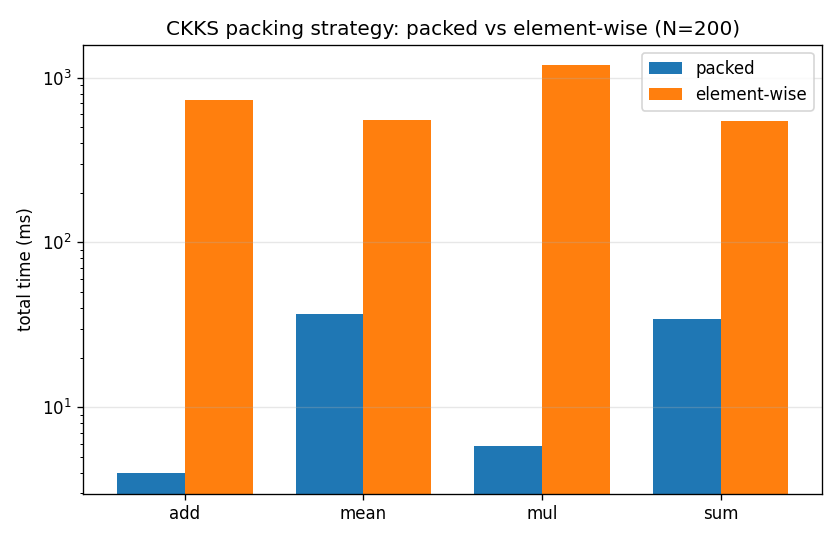
\includegraphics[width=0.72\linewidth]{packed_vs_elementwise.png}
\caption{Packed vs.\ element-wise total time, per operation, at $N=200$.}
\end{figure}

\subsection{The headline: computing on encrypted data, traditional vs.\ HE}

This is the comparison the project exists to make. \textbf{Scenario:} both sides
start from data \textbf{stored encrypted at rest} under their own scheme. To
compute an aggregate (here, \texttt{sum}) over that encrypted data:

\begin{itemize}[leftmargin=1.4em,itemsep=1pt]
  \item \textbf{Traditional (AES):} decrypt the dataset $\rightarrow$ compute on
    plaintext $\rightarrow$ (re-encrypt result). The data is \textbf{exposed in
    plaintext} to the compute party during the computation.
  \item \textbf{HE (CKKS), steady-state:} compute directly on the ciphertext,
    decrypt only the result. The data is \textbf{never exposed}. (A
    \emph{one-shot} variant additionally pays the CKKS encryption of the dataset
    --- the first upload to an untrusted cloud.)
\end{itemize}

\begin{table}[H]
\centering
\caption{Analytics cost for \texttt{sum} at $N=100{,}000$.}
\begin{tabularx}{\linewidth}{@{}Xcc@{}}
\toprule
\textbf{Workflow} & \textbf{Time for \texttt{sum}} & \textbf{Plaintext exposed?}\\
\midrule
AES: decrypt $+$ compute & \textbf{$\sim$0.16 ms} & \textbf{Yes}\\
HE steady-state: compute $+$ result decrypt & \textbf{$\sim$503 ms} ($\approx$576 ms one-shot incl.\ CKKS encryption) & \textbf{No}\\
\bottomrule
\end{tabularx}
\end{table}

\keyfinding{HE is roughly $3{,}000\times$ slower for this task. That number is
meaningless without its other half: the HE result was produced \emph{without the
compute party ever seeing the data.} The cost \emph{is} the security property.}

\begin{figure}[H]
\centering
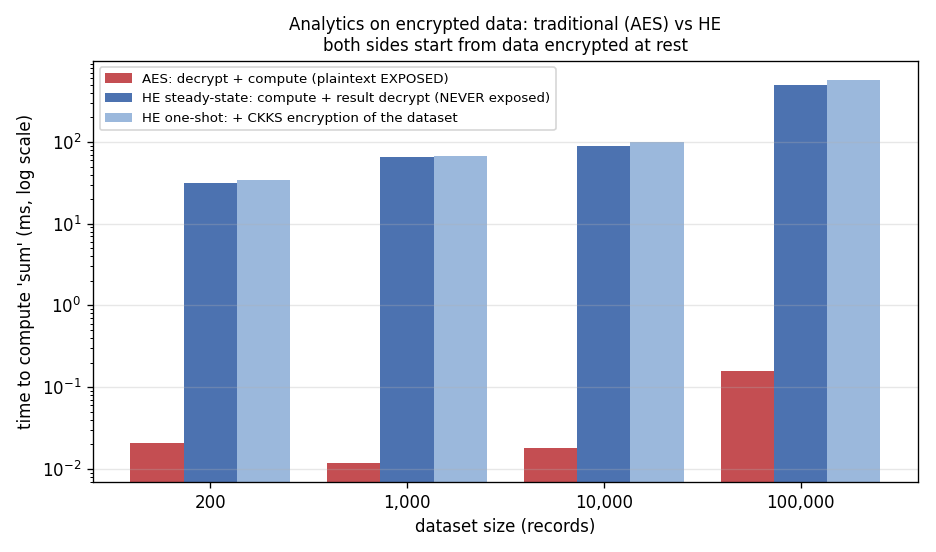
\includegraphics[width=0.72\linewidth]{workflow_comparison.png}
\caption{Analytics cost: AES (decrypt$+$compute) vs.\ HE steady-state and
one-shot.}
\end{figure}

\begin{figure}[H]
\centering
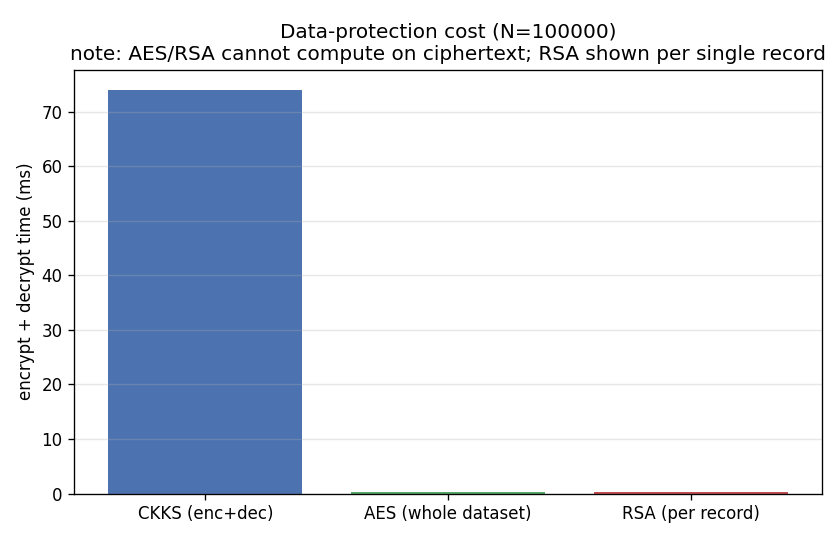
\includegraphics[width=0.72\linewidth]{protection_cost.png}
\caption{Whole-dataset encrypt$+$decrypt cost: CKKS vs.\ AES, plus RSA for a
single record.}
\end{figure}

\subsection{The measured depth limit}
\label{sec:depth}

HE is depth-limited, not merely slow --- and we measured the limit. Our parameter
chain \texttt{[60, 40, 40, 60]} provides two rescaling levels. A dedicated
experiment (\texttt{experiments/depth\_sweep.py}, repeated ciphertext-squaring of
unit-scale values) confirms it empirically:

\begin{table}[H]
\centering
\caption{CKKS error vs.\ multiplicative depth (repeated ct $\times$ ct squaring).}
\begin{tabular}{@{}clcc@{}}
\toprule
\textbf{Depth} & \textbf{Expr} & \textbf{Mean rel.\ error} & \textbf{Status}\\
\midrule
1 & $x^2$ & $\sim$$1.3\times10^{-7}$ & OK\\
2 & $x^4$ & $\sim$$9.4\times10^{-7}$ & OK\\
3 & $x^8$ & --- & \textbf{Fails: ``scale out of bounds''}\\
\bottomrule
\end{tabular}
\end{table}

The mean relative error grows $\sim$$7\times$ from depth 1 to depth 2, and a
third sequential multiplication \textbf{fails outright} --- the modulus chain is
exhausted. Deeper circuits require \emph{bootstrapping} (an expensive
noise-refresh) or larger parameters (more cost and memory). Our benchmark
deliberately stays within this budget --- single multiplications --- which is why
the multiply error stays at $\sim$$10^{-7}$ rather than diverging.

\begin{figure}[H]
\centering
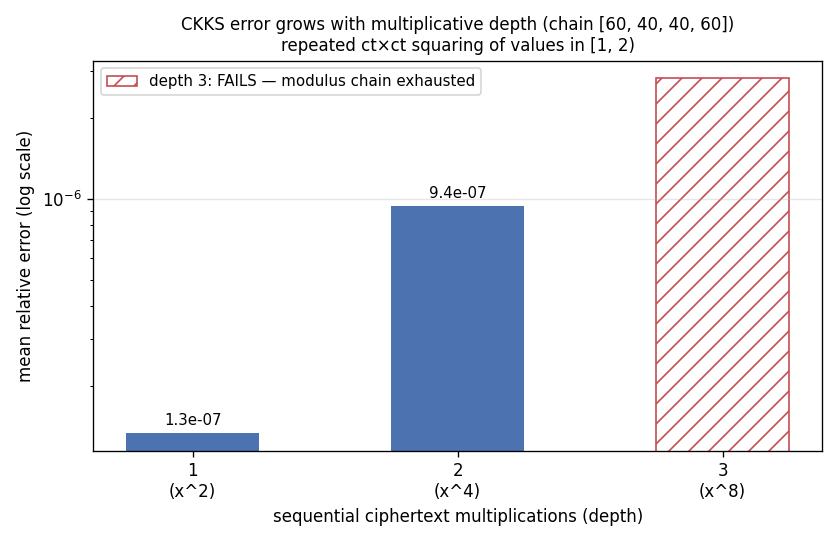
\includegraphics[width=0.72\linewidth]{ckks_error_vs_depth.png}
\caption{Measured CKKS error per multiplicative depth, and the depth-3 failure.}
\end{figure}

% ============================================================================
\section{Security Analysis}

Performance is only half of the assignment; the schemes also differ fundamentally
in what they secure.

\begin{table}[H]
\centering
\caption{Qualitative security profiles.}
\begin{tabularx}{\linewidth}{@{}p{2.1cm} >{\raggedright\arraybackslash}X >{\centering\arraybackslash}p{1.7cm} >{\centering\arraybackslash}p{1.7cm} >{\raggedright\arraybackslash}p{2.5cm}@{}}
\toprule
\textbf{Scheme} & \textbf{Type / security} & \textbf{Compute on ct?} & \textbf{Protects in use?} & \textbf{Quantum}\\
\midrule
AES-256-GCM   & Symmetric AEAD, $\sim$256-bit ($\sim$128 vs.\ Grover) & No & No & Resists Grover\\
RSA-2048-OAEP & Asymmetric, $\sim$112-bit (NIST) & No & No & \textbf{Broken by Shor}\\
CKKS (TenSEAL)& Homomorphic (RLWE lattice), $\sim$128-bit & \textbf{Yes} & \textbf{Yes} & Believed quantum-resistant\\
\bottomrule
\end{tabularx}
\end{table}

\textbf{HE's unique security benefit} is protecting data \emph{in use}: an
untrusted server can compute on ciphertext it cannot read. Two honest
qualifications keep this from being overstated:

\begin{itemize}[leftmargin=1.4em,itemsep=1pt]
  \item \textbf{Scope of protection.} AES-GCM also provides
    integrity/authenticity; CKKS provides confidentiality only and is
    approximate, so results carry (measured) error and integrity must be added
    separately (e.g.\ verifiable computation) if required.
  \item \textbf{Approximate-decryption caveat.} For CKKS specifically, releasing
    decrypted approximate results to an adversary can leak information about the
    secret key (Li \& Micciancio, 2021); this is mitigated by noise flooding
    before sharing decryptions.
\end{itemize}

On the quantum axis, CKKS (lattice/RLWE) is a post-quantum candidate and
RSA-2048 is not, a genuine point in HE's favour beyond the in-use property.

% ============================================================================
\section{Discussion and Insights --- When Is HE Practical?}

The measurements support a clear, bounded recommendation.

\textbf{HE is worth the cost when} the requirement is precisely \emph{``compute on
data the compute party must never see''} --- for example, analytics outsourced to
an untrusted cloud, or aggregation across parties that cannot share raw data ---
and when the workload tolerates a $\sim$$10^{2}$--$10^{3}\times$ slowdown and
$\sim$$10\times$ data inflation. Our errors confirm the results remain accurate
enough for such analytics.

\textbf{HE is impractical when} latency or footprint dominate. Three measured
reasons:
\begin{enumerate}[leftmargin=1.4em,itemsep=1pt]
  \item \textbf{The fixed $\sim$\SI{34}{\mega\byte} key/context overhead} makes
    small or per-request workloads absurd --- for 200 records the keys dwarf the
    data $\sim$$100\times$.
  \item \textbf{Packing is mandatory.} Without batching, both time and size blow
    up $\sim$$200\times$; element-wise use is effectively unusable.
  \item \textbf{HE is depth-limited, not merely slow} (\S\ref{sec:depth}): two
    multiplications, then the modulus chain is exhausted. It suits shallow
    analytics (sums, averages, single products), not arbitrary deep computation,
    without further machinery.
\end{enumerate}

The overarching insight is that the headline ``$3{,}000\times$ slower'' number,
quoted alone, is a caricature. Read against its security property and its
operating envelope --- shallow, batched, real-valued aggregation over data that
must never be decrypted by the compute party --- HE is not a slower AES but a
different tool that AES cannot replace.

% ============================================================================
\section{Deliverables}

The project produced a single reproducible artifact with the following
components:

\begin{itemize}[leftmargin=1.4em,itemsep=1pt]
  \item \textbf{Benchmark codebase} --- CKKS HE pipeline, AES/RSA baselines,
    seeded data generator, plaintext reference, and measurement harness
    (\texttt{he\_benchmark/}, \texttt{experiments/}).
  \item \textbf{Measured results} --- \texttt{results/results.csv}
    (48 rows: every scheme $\times$ operation $\times$ size, mean of 5 repeats),
    \texttt{results/depth\_sweep.json}, \texttt{results/workflow\_comparison.csv},
    and \texttt{results/run\_config.json} (environment + parameters).
  \item \textbf{Eight figures} --- runtime, cost breakdown, ciphertext size,
    error vs.\ size, error vs.\ depth, packed vs.\ element-wise, protection cost,
    and the workflow comparison (\texttt{figures/}).
  \item \textbf{Interactive dashboard} --- a 4-tab Streamlit app (dashboard,
    live HE demo, confidential use case, security \& traditional-vs-HE
    comparison) that reuses the benchmark modules so live results match the
    measured pipeline.
  \item \textbf{Test suite} --- 21 pytest tests (correctness, metrics layer,
    security invariants, headless app smoke tests).
  \item \textbf{Reproducible environment} --- Docker image, \texttt{docker-compose},
    and a pinned \texttt{requirements.lock}.
  \item \textbf{Written report} --- this document (and a Markdown/DOCX variant),
    plus a self-contained \texttt{PROJECT\_OVERVIEW.md}.
\end{itemize}

The one item not yet built is a final presentation deck.

% ============================================================================
\section{Testing and Verification}

Correctness is not asserted; it is tested. The suite of \textbf{21 pytest tests}
covers: CKKS correctness (packed and element-wise; sum/mean/add/mul; chunking
above one ciphertext; a multi-chunk vector round-trip that pins element
\emph{order}), the measurement layer itself (warm-up discarding, sub-ms batch
sizing, sampler sanity), AES/RSA round-trips, security-profile invariants, and
headless Streamlit \texttt{AppTest} smoke tests that run the app and exercise the
live-demo and use-case buttons.

A reproducible run (\texttt{docker compose run --rm benchmark}) regenerates the
CSV and run-config, verified across all four sizes with all operations correct.
The smoke tests earned their place by catching a real version bug
(\texttt{st.image(use\_container\_width=...)}, invalid in Streamlit 1.37, fixed to
\texttt{use\_column\_width}).

% ============================================================================
\section{How to Run}

The Docker image is the canonical environment; every command below is
reproducible from a clean checkout.

\begin{lstlisting}[caption={Reproduction commands.},captionpos=b]
docker compose build                             # build the image
docker compose run --rm benchmark pytest -v      # 21 correctness tests
docker compose run --rm benchmark                # -> results/results.csv + run_config.json
docker compose run --rm benchmark \
    python experiments/depth_sweep.py            # -> results/depth_sweep.json
docker compose run --rm plots                    # -> figures/*.png
docker compose up dashboard                      # interactive UI at http://localhost:8501
\end{lstlisting}

All numbers in this report are derived from \texttt{results/results.csv} and
\texttt{results/depth\_sweep.json}; CKKS parameters and environment are recorded
in \texttt{results/run\_config.json}.

% ============================================================================
\section{Limitations}
\label{sec:limitations}

\begin{itemize}[leftmargin=1.4em,itemsep=1pt]
  \item \textbf{Synthetic data.} We benchmark uniform-random \texttt{float64}
    arrays, not a named real-world dataset. The pipeline is dataset-agnostic;
    substituting a real numeric dataset is straightforward and is future work.
  \item \textbf{Process memory not reported as a headline.} We sampled process
    resident-set size (RSS) via psutil (not \texttt{tracemalloc}, which cannot
    see TenSEAL's C++ allocations), but RSS deltas are unreliable for short
    operations (freed pages are reused). We therefore treat \textbf{ciphertext
    size plus the fixed key/context size} as the authoritative memory signal; the
    raw RSS column stays in the CSV but no RSS figure is generated.
  \item \textbf{CKKS only.} We did not implement BFV/BGV. Exact integer
    \texttt{sum}/\texttt{count} under BFV would complement CKKS's approximate real
    arithmetic and is the most natural next step.
  \item \textbf{Element-wise capped at $N\approx200$.} Element-wise encryption
    exhausts container memory above that size; the packed path runs to
    \num{100000}.
\end{itemize}

% ============================================================================
\section{Conclusion and Future Work}

We built a reproducible benchmark that runs four numerical operations under CKKS
HE and under AES-256/RSA-2048 baselines, verifies every HE result against a
plaintext reference, and measures runtime, ciphertext size, approximation error,
and scalability to \num{100000} records. The central, honest finding is that HE
buys a capability the baselines lack --- computation on encrypted data, with data
never exposed in use --- at a measured cost of roughly three orders of magnitude
in time, $\sim$$10\times$ in ciphertext size, a fixed $\sim$\SI{34}{\mega\byte} of
keys, and a measured hard limit of two multiplications before the modulus chain
is exhausted. Whether that trade is acceptable depends entirely on whether
protecting data \emph{in use} is a requirement.

\textbf{Future work:} add BFV for exact integer aggregation; benchmark a real
public numeric dataset; explore deeper circuits with bootstrapping and
alternative parameter sets; and evaluate GPU-accelerated HE backends.

% ============================================================================
\begin{thebibliography}{9}
\bibitem{ckks} J.~H. Cheon, A.~Kim, M.~Kim, Y.~Song.
  \emph{Homomorphic Encryption for Arithmetic of Approximate Numbers (CKKS).}
  ASIACRYPT 2017.
\bibitem{tenseal} A.~Benaissa, B.~Retiat, B.~Cebere, A.~E. Belfedhal.
  \emph{TenSEAL: A Library for Encrypted Tensor Operations Using Homomorphic
  Encryption.} 2021.
\bibitem{hestd} M.~Albrecht et al.
  \emph{Homomorphic Encryption Security Standard.}
  HomomorphicEncryption.org, 2018.
\bibitem{nist} National Institute of Standards and Technology.
  \emph{SP 800-57 Part 1 Rev.\ 5: Recommendation for Key Management.} 2020.
\bibitem{limicc} B.~Li, D.~Micciancio.
  \emph{On the Security of Homomorphic Encryption on Approximate Numbers.}
  EUROCRYPT 2021.
\bibitem{fips197} NIST. \emph{FIPS 197: Advanced Encryption Standard (AES).} 2001.
\bibitem{pkcs1} K.~Moriarty et al.
  \emph{PKCS \#1 v2.2 / RFC 8017: RSA Cryptography Specifications.} 2016.
\end{thebibliography}

% ============================================================================
\appendix
\section{Baseline Reference Numbers}

\begin{itemize}[leftmargin=1.4em,itemsep=1pt]
  \item \textbf{AES-256-GCM}, protect (encrypt $+$ decrypt), total:
    0.030~ms ($N=200$), 0.018~ms (1k), 0.033~ms (10k), 0.330~ms (100k);
    ciphertext size $= N\times8 + 28$ bytes.
  \item \textbf{RSA-2048-OAEP}, per single 8-byte record: $\sim$0.02~ms encrypt,
    $\sim$0.20~ms decrypt; ciphertext 256 bytes per record. Bulk data would use
    hybrid encryption (RSA wraps an AES key).
  \item \emph{Reading these numbers:} they are microseconds, near
    \texttt{perf\_counter}'s practical noise floor at five repeats --- the
    non-monotonicity across sizes (1k faster than 200) is timing jitter, not a
    real effect. The harness batches sub-millisecond calls per timing sample to
    suppress exactly this.
\end{itemize}

\end{document}
